\documentclass[1p]{elsarticle_modified}
%\bibliographystyle{elsarticle-num}

%\usepackage[colorlinks]{hyperref}
%\usepackage{abbrmath_seonhwa} %\Abb, \Ascr, \Acal ,\Abf, \Afrak
\usepackage{amsfonts}
\usepackage{amssymb}
\usepackage{amsmath}
\usepackage{amsthm}
\usepackage{scalefnt}
\usepackage{amsbsy}
\usepackage{kotex}
\usepackage{caption}
\usepackage{subfig}
\usepackage{color}
\usepackage{graphicx}
\usepackage{xcolor} %% white, black, red, green, blue, cyan, magenta, yellow
\usepackage{float}
\usepackage{setspace}
\usepackage{hyperref}

\usepackage{tikz}
\usetikzlibrary{arrows}

\usepackage{multirow}
\usepackage{array} % fixed length table
\usepackage{hhline}

%%%%%%%%%%%%%%%%%%%%%
\makeatletter
\renewcommand*\env@matrix[1][\arraystretch]{%
	\edef\arraystretch{#1}%
	\hskip -\arraycolsep
	\let\@ifnextchar\new@ifnextchar
	\array{*\c@MaxMatrixCols c}}
\makeatother %https://tex.stackexchange.com/questions/14071/how-can-i-increase-the-line-spacing-in-a-matrix
%%%%%%%%%%%%%%%

\usepackage[normalem]{ulem}

\newcommand{\msout}[1]{\ifmmode\text{\sout{\ensuremath{#1}}}\else\sout{#1}\fi}
%SOURCE: \msout is \stkout macro in https://tex.stackexchange.com/questions/20609/strikeout-in-math-mode

\newcommand{\cancel}[1]{
	\ifmmode
	{\color{red}\msout{#1}}
	\else
	{\color{red}\sout{#1}}
	\fi
}

\newcommand{\add}[1]{
	{\color{blue}\uwave{#1}}
}

\newcommand{\replace}[2]{
	\ifmmode
	{\color{red}\msout{#1}}{\color{blue}\uwave{#2}}
	\else
	{\color{red}\sout{#1}}{\color{blue}\uwave{#2}}
	\fi
}

\newcommand{\Sol}{\mathcal{S}} %segment
\newcommand{\D}{D} %diagram
\newcommand{\A}{\mathcal{A}} %arc


%%%%%%%%%%%%%%%%%%%%%%%%%%%%%5 test

\def\sl{\operatorname{\textup{SL}}(2,\Cbb)}
\def\psl{\operatorname{\textup{PSL}}(2,\Cbb)}
\def\quan{\mkern 1mu \triangleright \mkern 1mu}

\theoremstyle{definition}
\newtheorem{thm}{Theorem}[section]
\newtheorem{prop}[thm]{Proposition}
\newtheorem{lem}[thm]{Lemma}
\newtheorem{ques}[thm]{Question}
\newtheorem{cor}[thm]{Corollary}
\newtheorem{defn}[thm]{Definition}
\newtheorem{exam}[thm]{Example}
\newtheorem{rmk}[thm]{Remark}
\newtheorem{alg}[thm]{Algorithm}

\newcommand{\I}{\sqrt{-1}}
\begin{document}

%\begin{frontmatter}
%
%\title{Boundary parabolic representations of knots up to 8 crossings}
%
%%% Group authors per affiliation:
%\author{Yunhi Cho} 
%\address{Department of Mathematics, University of Seoul, Seoul, Korea}
%\ead{yhcho@uos.ac.kr}
%
%
%\author{Seonhwa Kim} %\fnref{s_kim}}
%\address{Center for Geometry and Physics, Institute for Basic Science, Pohang, 37673, Korea}
%\ead{ryeona17@ibs.re.kr}
%
%\author{Hyuk Kim}
%\address{Department of Mathematical Sciences, Seoul National University, Seoul 08826, Korea}
%\ead{hyukkim@snu.ac.kr}
%
%\author{Seokbeom Yoon}
%\address{Department of Mathematical Sciences, Seoul National University, Seoul, 08826,  Korea}
%\ead{sbyoon15@snu.ac.kr}
%
%\begin{abstract}
%We find all boundary parabolic representation of knots up to 8 crossings.
%
%\end{abstract}
%\begin{keyword}
%    \MSC[2010] 57M25 
%\end{keyword}
%
%\end{frontmatter}

%\linenumbers
%\tableofcontents
%
\newcommand\colored[1]{\textcolor{white}{\rule[-0.35ex]{0.8em}{1.4ex}}\kern-0.8em\color{red} #1}%
%\newcommand\colored[1]{\textcolor{white}{ #1}\kern-2.17ex	\textcolor{white}{ #1}\kern-1.81ex	\textcolor{white}{ #1}\kern-2.15ex\color{red}#1	}

{\Large $\underline{12a_{1073}~(K12a_{1073})}$}

\setlength{\tabcolsep}{10pt}
\renewcommand{\arraystretch}{1.6}
\vspace{1cm}\begin{tabular}{m{100pt}>{\centering\arraybackslash}m{274pt}}
\multirow{5}{120pt}{
	\centering
	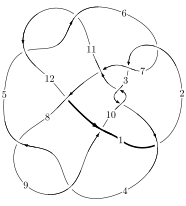
\includegraphics[width=112pt]{../../../GIT/diagram.site/Diagrams/png/1874_12a_1073.png}\\
\ \ \ A knot diagram\footnotemark}&
\allowdisplaybreaks
\textbf{Linearized knot diagam} \\
\cline{2-2}
 &
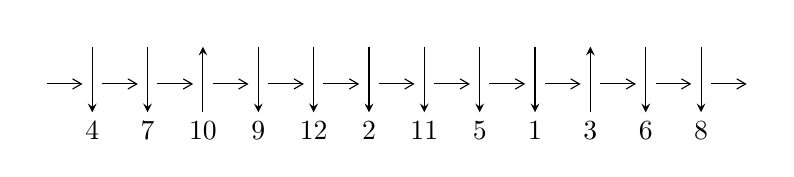
\begin{tikzpicture}[x=20pt, y=17pt]
	% nodes
	\node (C0) at (0, 0) {};
	\node (C1) at (1, 0) {};
	\node (C1U) at (1, +1) {};
	\node (C1D) at (1, -1) {4};

	\node (C2) at (2, 0) {};
	\node (C2U) at (2, +1) {};
	\node (C2D) at (2, -1) {7};

	\node (C3) at (3, 0) {};
	\node (C3U) at (3, +1) {};
	\node (C3D) at (3, -1) {10};

	\node (C4) at (4, 0) {};
	\node (C4U) at (4, +1) {};
	\node (C4D) at (4, -1) {9};

	\node (C5) at (5, 0) {};
	\node (C5U) at (5, +1) {};
	\node (C5D) at (5, -1) {12};

	\node (C6) at (6, 0) {};
	\node (C6U) at (6, +1) {};
	\node (C6D) at (6, -1) {2};

	\node (C7) at (7, 0) {};
	\node (C7U) at (7, +1) {};
	\node (C7D) at (7, -1) {11};

	\node (C8) at (8, 0) {};
	\node (C8U) at (8, +1) {};
	\node (C8D) at (8, -1) {5};

	\node (C9) at (9, 0) {};
	\node (C9U) at (9, +1) {};
	\node (C9D) at (9, -1) {1};

	\node (C10) at (10, 0) {};
	\node (C10U) at (10, +1) {};
	\node (C10D) at (10, -1) {3};

	\node (C11) at (11, 0) {};
	\node (C11U) at (11, +1) {};
	\node (C11D) at (11, -1) {6};

	\node (C12) at (12, 0) {};
	\node (C12U) at (12, +1) {};
	\node (C12D) at (12, -1) {8};
	\node (C13) at (13, 0) {};

	% arrows
	\draw[->,>={angle 60}]
	(C0) edge (C1) (C1) edge (C2) (C2) edge (C3) (C3) edge (C4) (C4) edge (C5) (C5) edge (C6) (C6) edge (C7) (C7) edge (C8) (C8) edge (C9) (C9) edge (C10) (C10) edge (C11) (C11) edge (C12) (C12) edge (C13) ;	\draw[->,>=stealth]
	(C1U) edge (C1D) (C2U) edge (C2D) (C3D) edge (C3U) (C4U) edge (C4D) (C5U) edge (C5D) (C6U) edge (C6D) (C7U) edge (C7D) (C8U) edge (C8D) (C9U) edge (C9D) (C10D) edge (C10U) (C11U) edge (C11D) (C12U) edge (C12D) ;
	\end{tikzpicture} \\
\hhline{~~} \\& 
\textbf{Solving Sequence} \\ \cline{2-2} 
 &
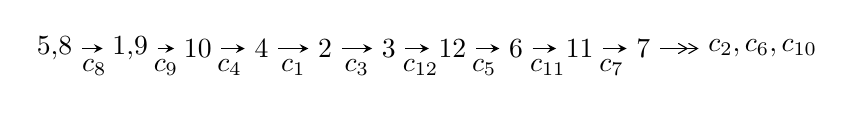
\begin{tikzpicture}[x=23pt, y=7pt]
	% node
	\node (A0) at (-1/8, 0) {5,8};
	\node (A1) at (17/16, 0) {1,9};
	\node (A2) at (17/8, 0) {10};
	\node (A3) at (25/8, 0) {4};
	\node (A4) at (33/8, 0) {2};
	\node (A5) at (41/8, 0) {3};
	\node (A6) at (49/8, 0) {12};
	\node (A7) at (57/8, 0) {6};
	\node (A8) at (65/8, 0) {11};
	\node (A9) at (73/8, 0) {7};
	\node (C1) at (1/2, -1) {$c_{8}$};
	\node (C2) at (13/8, -1) {$c_{9}$};
	\node (C3) at (21/8, -1) {$c_{4}$};
	\node (C4) at (29/8, -1) {$c_{1}$};
	\node (C5) at (37/8, -1) {$c_{3}$};
	\node (C6) at (45/8, -1) {$c_{12}$};
	\node (C7) at (53/8, -1) {$c_{5}$};
	\node (C8) at (61/8, -1) {$c_{11}$};
	\node (C9) at (69/8, -1) {$c_{7}$};
	\node (A10) at (11, 0) {$c_{2},c_{6},c_{10}$};

	% edge
	\draw[->,>=stealth]	
	(A0) edge (A1) (A1) edge (A2) (A2) edge (A3) (A3) edge (A4) (A4) edge (A5) (A5) edge (A6) (A6) edge (A7) (A7) edge (A8) (A8) edge (A9) ;
	\draw[->>,>={angle 60}]	
	(A9) edge (A10);
\end{tikzpicture} \\ 

\end{tabular} \\

\footnotetext{
The image of knot diagram is generated by the software ``\textbf{Draw programme}" developed by Andrew Bartholomew(\url{http://www.layer8.co.uk/maths/draw/index.htm\#Running-draw}), where we modified some parts for our purpose(\url{https://github.com/CATsTAILs/LinksPainter}).
}\phantom \\ \newline 
\centering \textbf{Ideals for irreducible components\footnotemark of $X_{\text{par}}$} 
 
\begin{align*}
I^u_{1}&=\langle 
2.54817\times10^{592} u^{140}+1.63249\times10^{593} u^{139}+\cdots+1.25499\times10^{594} b+3.83199\times10^{594},\\
\phantom{I^u_{1}}&\phantom{= \langle  }-4.59910\times10^{593} u^{140}-3.23099\times10^{594} u^{139}+\cdots+1.50598\times10^{595} a-1.02194\times10^{597},\\
\phantom{I^u_{1}}&\phantom{= \langle  }u^{141}+4 u^{140}+\cdots+2832 u+168\rangle \\
I^u_{2}&=\langle 
6.58267\times10^{20} u^{31}+6.86615\times10^{21} u^{30}+\cdots+2.03894\times10^{21} b+2.89056\times10^{23},\\
\phantom{I^u_{2}}&\phantom{= \langle  }-9.29799\times10^{22} u^{31}-4.19012\times10^{23} u^{30}+\cdots+1.20297\times10^{23} a-2.06819\times10^{25},\\
\phantom{I^u_{2}}&\phantom{= \langle  }u^{32}- u^{31}+\cdots-104 u+59\rangle \\
\\
I^v_{1}&=\langle 
a,\;b-1,\;v^3+2 v+1\rangle \\
\end{align*}
\raggedright * 3 irreducible components of $\dim_{\mathbb{C}}=0$, with total 176 representations.\\
\footnotetext{All coefficients of polynomials are rational numbers. But the coefficients are sometimes approximated in decimal forms when there is not enough margin.}
\newpage
\renewcommand{\arraystretch}{1}
\centering \section*{I. $I^u_{1}= \langle 2.55\times10^{592} u^{140}+1.63\times10^{593} u^{139}+\cdots+1.25\times10^{594} b+3.83\times10^{594},\;-4.60\times10^{593} u^{140}-3.23\times10^{594} u^{139}+\cdots+1.51\times10^{595} a-1.02\times10^{597},\;u^{141}+4 u^{140}+\cdots+2832 u+168 \rangle$}
\flushleft \textbf{(i) Arc colorings}\\
\begin{tabular}{m{7pt} m{180pt} m{7pt} m{180pt} }
\flushright $a_{5}=$&$\begin{pmatrix}0\\u\end{pmatrix}$ \\
\flushright $a_{8}=$&$\begin{pmatrix}1\\0\end{pmatrix}$ \\
\flushright $a_{1}=$&$\begin{pmatrix}0.0305389 u^{140}+0.214544 u^{139}+\cdots+476.782 u+67.8590\\-0.0203043 u^{140}-0.130081 u^{139}+\cdots-86.0127 u-3.05341\end{pmatrix}$ \\
\flushright $a_{9}=$&$\begin{pmatrix}1\\u^2\end{pmatrix}$ \\
\flushright $a_{10}=$&$\begin{pmatrix}-0.0126430 u^{140}+0.0241027 u^{139}+\cdots+167.192 u-2.57404\\0.0411553 u^{140}+0.137220 u^{139}+\cdots-52.7399 u-4.70944\end{pmatrix}$ \\
\flushright $a_{4}=$&$\begin{pmatrix}u\\u^3+u\end{pmatrix}$ \\
\flushright $a_{2}=$&$\begin{pmatrix}0.00790478 u^{140}+0.100131 u^{139}+\cdots+430.040 u+65.5289\\-0.0187936 u^{140}-0.115024 u^{139}+\cdots-61.3348 u-1.37233\end{pmatrix}$ \\
\flushright $a_{3}=$&$\begin{pmatrix}-0.0198734 u^{140}+0.0433603 u^{139}+\cdots+208.509 u+20.4485\\-0.0123183 u^{140}-0.108437 u^{139}+\cdots-107.608 u-5.43547\end{pmatrix}$ \\
\flushright $a_{12}=$&$\begin{pmatrix}0.0102345 u^{140}+0.0844631 u^{139}+\cdots+390.769 u+64.8056\\-0.0203043 u^{140}-0.130081 u^{139}+\cdots-86.0127 u-3.05341\end{pmatrix}$ \\
\flushright $a_{6}=$&$\begin{pmatrix}-0.0488240 u^{140}-0.150140 u^{139}+\cdots+351.967 u+29.9572\\-0.0878505 u^{140}-0.280169 u^{139}+\cdots+157.323 u+9.17097\end{pmatrix}$ \\
\flushright $a_{11}=$&$\begin{pmatrix}-0.116715 u^{140}-0.443627 u^{139}+\cdots+54.4349 u-12.8563\\0.00779702 u^{140}+0.0699302 u^{139}+\cdots+64.1007 u+1.77825\end{pmatrix}$ \\
\flushright $a_{7}=$&$\begin{pmatrix}-0.0774632 u^{140}-0.271390 u^{139}+\cdots-30.5227 u-33.3656\\0.00340777 u^{140}+0.0631506 u^{139}+\cdots+85.7404 u+2.52528\end{pmatrix}$\\&\end{tabular}
\flushleft \textbf{(ii) Obstruction class $= -1$}\\~\\
\flushleft \textbf{(iii) Cusp Shapes $= -0.143156 u^{140}-0.698212 u^{139}+\cdots-254.819 u-13.1150$}\\~\\
\newpage\renewcommand{\arraystretch}{1}
\flushleft \textbf{(iv) u-Polynomials at the component}\newline \\
\begin{tabular}{m{50pt}|m{274pt}}
Crossings & \hspace{64pt}u-Polynomials at each crossing \\
\hline $$\begin{aligned}c_{1}\end{aligned}$$&$\begin{aligned}
&u^{141}-12 u^{140}+\cdots+763 u-49
\end{aligned}$\\
\hline $$\begin{aligned}c_{2},c_{6}\end{aligned}$$&$\begin{aligned}
&u^{141}-2 u^{140}+\cdots+45051 u+32979
\end{aligned}$\\
\hline $$\begin{aligned}c_{3},c_{10}\end{aligned}$$&$\begin{aligned}
&u^{141}+u^{140}+\cdots+386164 u+65629
\end{aligned}$\\
\hline $$\begin{aligned}c_{4},c_{8}\end{aligned}$$&$\begin{aligned}
&u^{141}+4 u^{140}+\cdots+2832 u+168
\end{aligned}$\\
\hline $$\begin{aligned}c_{5},c_{11}\end{aligned}$$&$\begin{aligned}
&u^{141}- u^{140}+\cdots+533427 u+47167
\end{aligned}$\\
\hline $$\begin{aligned}c_{7}\end{aligned}$$&$\begin{aligned}
&u^{141}+8 u^{140}+\cdots+47275162 u+6401042
\end{aligned}$\\
\hline $$\begin{aligned}c_{9}\end{aligned}$$&$\begin{aligned}
&u^{141}+8 u^{140}+\cdots+26 u+1
\end{aligned}$\\
\hline $$\begin{aligned}c_{12}\end{aligned}$$&$\begin{aligned}
&u^{141}-2 u^{140}+\cdots+14863691 u+980999
\end{aligned}$\\
\hline
\end{tabular}\\~\\
\newpage\renewcommand{\arraystretch}{1}
\flushleft \textbf{(v) Riley Polynomials at the component}\newline \\
\begin{tabular}{m{50pt}|m{274pt}}
Crossings & \hspace{64pt}Riley Polynomials at each crossing \\
\hline $$\begin{aligned}c_{1}\end{aligned}$$&$\begin{aligned}
&y^{141}-2 y^{140}+\cdots-122941 y-2401
\end{aligned}$\\
\hline $$\begin{aligned}c_{2},c_{6}\end{aligned}$$&$\begin{aligned}
&y^{141}-84 y^{140}+\cdots+18315150465 y-1087614441
\end{aligned}$\\
\hline $$\begin{aligned}c_{3},c_{10}\end{aligned}$$&$\begin{aligned}
&y^{141}+119 y^{140}+\cdots+200837368090 y-4307165641
\end{aligned}$\\
\hline $$\begin{aligned}c_{4},c_{8}\end{aligned}$$&$\begin{aligned}
&y^{141}+110 y^{140}+\cdots+8842080 y-28224
\end{aligned}$\\
\hline $$\begin{aligned}c_{5},c_{11}\end{aligned}$$&$\begin{aligned}
&y^{141}+107 y^{140}+\cdots-15637743751 y-2224725889
\end{aligned}$\\
\hline $$\begin{aligned}c_{7}\end{aligned}$$&$\begin{aligned}
&y^{141}-40 y^{140}+\cdots-12502874859103792 y-40973338685764
\end{aligned}$\\
\hline $$\begin{aligned}c_{9}\end{aligned}$$&$\begin{aligned}
&y^{141}-6 y^{140}+\cdots+136 y-1
\end{aligned}$\\
\hline $$\begin{aligned}c_{12}\end{aligned}$$&$\begin{aligned}
&y^{141}+58 y^{140}+\cdots-23268885446441 y-962359038001
\end{aligned}$\\
\hline
\end{tabular}\\~\\
\newpage\flushleft \textbf{(vi) Complex Volumes and Cusp Shapes}
$$\begin{array}{c|c|c}  
\text{Solutions to }I^u_{1}& \I (\text{vol} + \sqrt{-1}CS) & \text{Cusp shape}\\
 \hline 
\begin{aligned}
u &= -0.763169 + 0.633004 I \\
a &= -1.339640 + 0.080630 I \\
b &= \phantom{-}0.715686 + 1.075370 I\end{aligned}
 & -3.45255 - 4.17755 I & \phantom{-0.000000 } 0 \\ \hline\begin{aligned}
u &= -0.763169 - 0.633004 I \\
a &= -1.339640 - 0.080630 I \\
b &= \phantom{-}0.715686 - 1.075370 I\end{aligned}
 & -3.45255 + 4.17755 I & \phantom{-0.000000 } 0 \\ \hline\begin{aligned}
u &= \phantom{-}0.155407 + 1.012010 I \\
a &= \phantom{-}0.49435 + 1.78486 I \\
b &= -0.497754 - 0.766992 I\end{aligned}
 & -1.79602 - 1.77015 I & \phantom{-0.000000 } 0 \\ \hline\begin{aligned}
u &= \phantom{-}0.155407 - 1.012010 I \\
a &= \phantom{-}0.49435 - 1.78486 I \\
b &= -0.497754 + 0.766992 I\end{aligned}
 & -1.79602 + 1.77015 I & \phantom{-0.000000 } 0 \\ \hline\begin{aligned}
u &= -0.340769 + 0.969240 I \\
a &= -0.50551 - 2.16701 I \\
b &= -0.80000 + 2.24860 I\end{aligned}
 & -2.47493 + 8.56476 I & \phantom{-0.000000 } 0 \\ \hline\begin{aligned}
u &= -0.340769 - 0.969240 I \\
a &= -0.50551 + 2.16701 I \\
b &= -0.80000 - 2.24860 I\end{aligned}
 & -2.47493 - 8.56476 I & \phantom{-0.000000 } 0 \\ \hline\begin{aligned}
u &= \phantom{-}0.986469 + 0.297194 I \\
a &= -0.143405 + 0.208271 I \\
b &= \phantom{-}0.837739 + 0.774239 I\end{aligned}
 & -1.60144 - 7.36841 I & \phantom{-0.000000 } 0 \\ \hline\begin{aligned}
u &= \phantom{-}0.986469 - 0.297194 I \\
a &= -0.143405 - 0.208271 I \\
b &= \phantom{-}0.837739 - 0.774239 I\end{aligned}
 & -1.60144 + 7.36841 I & \phantom{-0.000000 } 0 \\ \hline\begin{aligned}
u &= \phantom{-}0.939371 + 0.072087 I \\
a &= -0.063001 - 0.319054 I \\
b &= -1.046510 + 0.355654 I\end{aligned}
 & -9.05838 + 7.91895 I & \phantom{-0.000000 } 0 \\ \hline\begin{aligned}
u &= \phantom{-}0.939371 - 0.072087 I \\
a &= -0.063001 + 0.319054 I \\
b &= -1.046510 - 0.355654 I\end{aligned}
 & -9.05838 - 7.91895 I & \phantom{-0.000000 } 0\\
 \hline 
 \end{array}$$\newpage$$\begin{array}{c|c|c}  
\text{Solutions to }I^u_{1}& \I (\text{vol} + \sqrt{-1}CS) & \text{Cusp shape}\\
 \hline 
\begin{aligned}
u &= \phantom{-}0.843079 + 0.393632 I \\
a &= \phantom{-}0.564951 + 0.190127 I \\
b &= \phantom{-}0.664303 - 0.159681 I\end{aligned}
 & -1.86166 + 1.83381 I & \phantom{-0.000000 } 0 \\ \hline\begin{aligned}
u &= \phantom{-}0.843079 - 0.393632 I \\
a &= \phantom{-}0.564951 - 0.190127 I \\
b &= \phantom{-}0.664303 + 0.159681 I\end{aligned}
 & -1.86166 - 1.83381 I & \phantom{-0.000000 } 0 \\ \hline\begin{aligned}
u &= \phantom{-}0.996431 + 0.423590 I \\
a &= -0.100176 - 0.242191 I \\
b &= -0.546016 - 0.686876 I\end{aligned}
 & \phantom{-}2.74069 - 3.01528 I & \phantom{-0.000000 } 0 \\ \hline\begin{aligned}
u &= \phantom{-}0.996431 - 0.423590 I \\
a &= -0.100176 + 0.242191 I \\
b &= -0.546016 + 0.686876 I\end{aligned}
 & \phantom{-}2.74069 + 3.01528 I & \phantom{-0.000000 } 0 \\ \hline\begin{aligned}
u &= -0.164481 + 1.074710 I \\
a &= \phantom{-}0.84942 - 1.93739 I \\
b &= \phantom{-}0.129569 + 0.279132 I\end{aligned}
 & -2.95677 + 4.09152 I & \phantom{-0.000000 } 0 \\ \hline\begin{aligned}
u &= -0.164481 - 1.074710 I \\
a &= \phantom{-}0.84942 + 1.93739 I \\
b &= \phantom{-}0.129569 - 0.279132 I\end{aligned}
 & -2.95677 - 4.09152 I & \phantom{-0.000000 } 0 \\ \hline\begin{aligned}
u &= \phantom{-}0.277431 + 0.863792 I \\
a &= -0.70330 - 1.83929 I \\
b &= \phantom{-}0.993033 + 0.994671 I\end{aligned}
 & -6.56670 - 4.32297 I & \phantom{-0.000000 } 0 \\ \hline\begin{aligned}
u &= \phantom{-}0.277431 - 0.863792 I \\
a &= -0.70330 + 1.83929 I \\
b &= \phantom{-}0.993033 - 0.994671 I\end{aligned}
 & -6.56670 + 4.32297 I & \phantom{-0.000000 } 0 \\ \hline\begin{aligned}
u &= -0.822181 + 0.321499 I \\
a &= \phantom{-}0.721318 - 0.332401 I \\
b &= -0.519997 - 0.944704 I\end{aligned}
 & -1.21432 - 2.33038 I & \phantom{-0.000000 } 0 \\ \hline\begin{aligned}
u &= -0.822181 - 0.321499 I \\
a &= \phantom{-}0.721318 + 0.332401 I \\
b &= -0.519997 + 0.944704 I\end{aligned}
 & -1.21432 + 2.33038 I & \phantom{-0.000000 } 0\\
 \hline 
 \end{array}$$\newpage$$\begin{array}{c|c|c}  
\text{Solutions to }I^u_{1}& \I (\text{vol} + \sqrt{-1}CS) & \text{Cusp shape}\\
 \hline 
\begin{aligned}
u &= -0.041884 + 1.119270 I \\
a &= -0.180792 + 0.017170 I \\
b &= \phantom{-}1.68313 + 0.04851 I\end{aligned}
 & -0.992191 + 0.266056 I & \phantom{-0.000000 } 0 \\ \hline\begin{aligned}
u &= -0.041884 - 1.119270 I \\
a &= -0.180792 - 0.017170 I \\
b &= \phantom{-}1.68313 - 0.04851 I\end{aligned}
 & -0.992191 - 0.266056 I & \phantom{-0.000000 } 0 \\ \hline\begin{aligned}
u &= -0.410529 + 1.070460 I \\
a &= -0.408143 + 0.787586 I \\
b &= \phantom{-}0.803532 - 0.455460 I\end{aligned}
 & -1.83641 + 1.10256 I & \phantom{-0.000000 } 0 \\ \hline\begin{aligned}
u &= -0.410529 - 1.070460 I \\
a &= -0.408143 - 0.787586 I \\
b &= \phantom{-}0.803532 + 0.455460 I\end{aligned}
 & -1.83641 - 1.10256 I & \phantom{-0.000000 } 0 \\ \hline\begin{aligned}
u &= -0.039398 + 1.150010 I \\
a &= \phantom{-}0.46753 + 2.07817 I \\
b &= -0.142788 - 0.773798 I\end{aligned}
 & -2.16440 - 2.33593 I & \phantom{-0.000000 } 0 \\ \hline\begin{aligned}
u &= -0.039398 - 1.150010 I \\
a &= \phantom{-}0.46753 - 2.07817 I \\
b &= -0.142788 + 0.773798 I\end{aligned}
 & -2.16440 + 2.33593 I & \phantom{-0.000000 } 0 \\ \hline\begin{aligned}
u &= \phantom{-}1.144550 + 0.149559 I \\
a &= \phantom{-}0.430020 + 0.204811 I \\
b &= -0.256705 + 0.964339 I\end{aligned}
 & \phantom{-}0.13672 + 2.12290 I & \phantom{-0.000000 } 0 \\ \hline\begin{aligned}
u &= \phantom{-}1.144550 - 0.149559 I \\
a &= \phantom{-}0.430020 - 0.204811 I \\
b &= -0.256705 - 0.964339 I\end{aligned}
 & \phantom{-}0.13672 - 2.12290 I & \phantom{-0.000000 } 0 \\ \hline\begin{aligned}
u &= -0.834257 + 0.002736 I \\
a &= -0.262575 + 0.153090 I \\
b &= \phantom{-}0.874699 + 0.856528 I\end{aligned}
 & -7.10130 - 2.33210 I & \phantom{-0.000000 } 0 \\ \hline\begin{aligned}
u &= -0.834257 - 0.002736 I \\
a &= -0.262575 - 0.153090 I \\
b &= \phantom{-}0.874699 - 0.856528 I\end{aligned}
 & -7.10130 + 2.33210 I & \phantom{-0.000000 } 0\\
 \hline 
 \end{array}$$\newpage$$\begin{array}{c|c|c}  
\text{Solutions to }I^u_{1}& \I (\text{vol} + \sqrt{-1}CS) & \text{Cusp shape}\\
 \hline 
\begin{aligned}
u &= \phantom{-}0.002645 + 1.178370 I \\
a &= \phantom{-}0.78053 - 2.25107 I \\
b &= -1.76800 + 2.30851 I\end{aligned}
 & -0.26531 - 7.50044 I & \phantom{-0.000000 } 0 \\ \hline\begin{aligned}
u &= \phantom{-}0.002645 - 1.178370 I \\
a &= \phantom{-}0.78053 + 2.25107 I \\
b &= -1.76800 - 2.30851 I\end{aligned}
 & -0.26531 + 7.50044 I & \phantom{-0.000000 } 0 \\ \hline\begin{aligned}
u &= -1.171170 + 0.248839 I \\
a &= -0.128236 - 0.164334 I \\
b &= \phantom{-}0.761366 - 0.817171 I\end{aligned}
 & -5.1060 + 13.3388 I & \phantom{-0.000000 } 0 \\ \hline\begin{aligned}
u &= -1.171170 - 0.248839 I \\
a &= -0.128236 + 0.164334 I \\
b &= \phantom{-}0.761366 + 0.817171 I\end{aligned}
 & -5.1060 - 13.3388 I & \phantom{-0.000000 } 0 \\ \hline\begin{aligned}
u &= -0.790003 + 0.110290 I \\
a &= \phantom{-}0.167515 - 0.456463 I \\
b &= -1.057430 + 0.177318 I\end{aligned}
 & -4.77992 + 3.20333 I & \phantom{-0.000000 } 0 \\ \hline\begin{aligned}
u &= -0.790003 - 0.110290 I \\
a &= \phantom{-}0.167515 + 0.456463 I \\
b &= -1.057430 - 0.177318 I\end{aligned}
 & -4.77992 - 3.20333 I & \phantom{-0.000000 } 0 \\ \hline\begin{aligned}
u &= -1.198270 + 0.099250 I \\
a &= \phantom{-}0.248775 + 0.144482 I \\
b &= -0.231409 + 0.617685 I\end{aligned}
 & -0.667207 + 0.969556 I & \phantom{-0.000000 } 0 \\ \hline\begin{aligned}
u &= -1.198270 - 0.099250 I \\
a &= \phantom{-}0.248775 - 0.144482 I \\
b &= -0.231409 - 0.617685 I\end{aligned}
 & -0.667207 - 0.969556 I & \phantom{-0.000000 } 0 \\ \hline\begin{aligned}
u &= \phantom{-}0.165118 + 1.197910 I \\
a &= \phantom{-}0.193142 - 1.214250 I \\
b &= -0.303338 + 0.861689 I\end{aligned}
 & \phantom{-}3.55356 + 0.06503 I & \phantom{-0.000000 } 0 \\ \hline\begin{aligned}
u &= \phantom{-}0.165118 - 1.197910 I \\
a &= \phantom{-}0.193142 + 1.214250 I \\
b &= -0.303338 - 0.861689 I\end{aligned}
 & \phantom{-}3.55356 - 0.06503 I & \phantom{-0.000000 } 0\\
 \hline 
 \end{array}$$\newpage$$\begin{array}{c|c|c}  
\text{Solutions to }I^u_{1}& \I (\text{vol} + \sqrt{-1}CS) & \text{Cusp shape}\\
 \hline 
\begin{aligned}
u &= \phantom{-}0.280111 + 1.177070 I \\
a &= \phantom{-}0.01971 + 1.50168 I \\
b &= \phantom{-}0.101289 - 0.900632 I\end{aligned}
 & \phantom{-}1.85029 - 4.46678 I & \phantom{-0.000000 } 0 \\ \hline\begin{aligned}
u &= \phantom{-}0.280111 - 1.177070 I \\
a &= \phantom{-}0.01971 - 1.50168 I \\
b &= \phantom{-}0.101289 + 0.900632 I\end{aligned}
 & \phantom{-}1.85029 + 4.46678 I & \phantom{-0.000000 } 0 \\ \hline\begin{aligned}
u &= \phantom{-}0.115170 + 1.209580 I \\
a &= -0.00940 + 2.86333 I \\
b &= -0.85445 - 2.86153 I\end{aligned}
 & \phantom{-}4.26570 - 0.47439 I & \phantom{-0.000000 } 0 \\ \hline\begin{aligned}
u &= \phantom{-}0.115170 - 1.209580 I \\
a &= -0.00940 - 2.86333 I \\
b &= -0.85445 + 2.86153 I\end{aligned}
 & \phantom{-}4.26570 + 0.47439 I & \phantom{-0.000000 } 0 \\ \hline\begin{aligned}
u &= -0.776246 + 0.081534 I \\
a &= \phantom{-}0.444633 + 0.094869 I \\
b &= \phantom{-}0.352412 - 0.113169 I\end{aligned}
 & -1.104670 - 0.011032 I & \phantom{-0.000000 } 0 \\ \hline\begin{aligned}
u &= -0.776246 - 0.081534 I \\
a &= \phantom{-}0.444633 - 0.094869 I \\
b &= \phantom{-}0.352412 + 0.113169 I\end{aligned}
 & -1.104670 + 0.011032 I & \phantom{-0.000000 } 0 \\ \hline\begin{aligned}
u &= \phantom{-}0.437847 + 1.139360 I \\
a &= -0.20526 + 1.49045 I \\
b &= -0.530547 - 0.515869 I\end{aligned}
 & \phantom{-}0.57932 - 6.57678 I & \phantom{-0.000000 } 0 \\ \hline\begin{aligned}
u &= \phantom{-}0.437847 - 1.139360 I \\
a &= -0.20526 - 1.49045 I \\
b &= -0.530547 + 0.515869 I\end{aligned}
 & \phantom{-}0.57932 + 6.57678 I & \phantom{-0.000000 } 0 \\ \hline\begin{aligned}
u &= \phantom{-}0.048975 + 1.220130 I \\
a &= -0.60346 + 1.50138 I \\
b &= -0.623416 - 1.161700 I\end{aligned}
 & \phantom{-}7.21232 - 0.33115 I & \phantom{-0.000000 } 0 \\ \hline\begin{aligned}
u &= \phantom{-}0.048975 - 1.220130 I \\
a &= -0.60346 - 1.50138 I \\
b &= -0.623416 + 1.161700 I\end{aligned}
 & \phantom{-}7.21232 + 0.33115 I & \phantom{-0.000000 } 0\\
 \hline 
 \end{array}$$\newpage$$\begin{array}{c|c|c}  
\text{Solutions to }I^u_{1}& \I (\text{vol} + \sqrt{-1}CS) & \text{Cusp shape}\\
 \hline 
\begin{aligned}
u &= \phantom{-}0.767288 + 0.096580 I \\
a &= -0.632730 - 1.129660 I \\
b &= \phantom{-}0.664099 - 0.529863 I\end{aligned}
 & -0.443046 - 0.013493 I & \phantom{-0.000000 } 0 \\ \hline\begin{aligned}
u &= \phantom{-}0.767288 - 0.096580 I \\
a &= -0.632730 + 1.129660 I \\
b &= \phantom{-}0.664099 + 0.529863 I\end{aligned}
 & -0.443046 + 0.013493 I & \phantom{-0.000000 } 0 \\ \hline\begin{aligned}
u &= \phantom{-}0.223800 + 1.207940 I \\
a &= -0.84723 - 1.80670 I \\
b &= \phantom{-}0.532875 + 0.811679 I\end{aligned}
 & -4.58833 - 0.55821 I & \phantom{-0.000000 } 0 \\ \hline\begin{aligned}
u &= \phantom{-}0.223800 - 1.207940 I \\
a &= -0.84723 + 1.80670 I \\
b &= \phantom{-}0.532875 - 0.811679 I\end{aligned}
 & -4.58833 + 0.55821 I & \phantom{-0.000000 } 0 \\ \hline\begin{aligned}
u &= -0.391296 + 1.171130 I \\
a &= \phantom{-}0.23242 + 1.77284 I \\
b &= \phantom{-}0.81059 - 1.75306 I\end{aligned}
 & \phantom{-}1.52382 + 6.81151 I & \phantom{-0.000000 } 0 \\ \hline\begin{aligned}
u &= -0.391296 - 1.171130 I \\
a &= \phantom{-}0.23242 - 1.77284 I \\
b &= \phantom{-}0.81059 + 1.75306 I\end{aligned}
 & \phantom{-}1.52382 - 6.81151 I & \phantom{-0.000000 } 0 \\ \hline\begin{aligned}
u &= -0.345880 + 1.188710 I \\
a &= -0.53837 - 1.73904 I \\
b &= \phantom{-}0.14774 + 1.82262 I\end{aligned}
 & -2.44838 + 7.03398 I & \phantom{-0.000000 } 0 \\ \hline\begin{aligned}
u &= -0.345880 - 1.188710 I \\
a &= -0.53837 + 1.73904 I \\
b &= \phantom{-}0.14774 - 1.82262 I\end{aligned}
 & -2.44838 - 7.03398 I & \phantom{-0.000000 } 0 \\ \hline\begin{aligned}
u &= -0.092057 + 1.234850 I \\
a &= -0.495450 - 1.295560 I \\
b &= -0.852071 + 0.905712 I\end{aligned}
 & \phantom{-}5.26983 + 5.03199 I & \phantom{-0.000000 } 0 \\ \hline\begin{aligned}
u &= -0.092057 - 1.234850 I \\
a &= -0.495450 + 1.295560 I \\
b &= -0.852071 - 0.905712 I\end{aligned}
 & \phantom{-}5.26983 - 5.03199 I & \phantom{-0.000000 } 0\\
 \hline 
 \end{array}$$\newpage$$\begin{array}{c|c|c}  
\text{Solutions to }I^u_{1}& \I (\text{vol} + \sqrt{-1}CS) & \text{Cusp shape}\\
 \hline 
\begin{aligned}
u &= -0.455722 + 0.609100 I \\
a &= \phantom{-}1.60614 - 0.30820 I \\
b &= \phantom{-}0.731630 - 0.135976 I\end{aligned}
 & -4.22921 - 1.70726 I & \phantom{-0.000000 } 0 \\ \hline\begin{aligned}
u &= -0.455722 - 0.609100 I \\
a &= \phantom{-}1.60614 + 0.30820 I \\
b &= \phantom{-}0.731630 + 0.135976 I\end{aligned}
 & -4.22921 + 1.70726 I & \phantom{-0.000000 } 0 \\ \hline\begin{aligned}
u &= \phantom{-}0.118808 + 1.242040 I \\
a &= -0.42103 - 1.77039 I \\
b &= \phantom{-}1.43043 + 1.74539 I\end{aligned}
 & \phantom{-}7.72459 - 2.11932 I & \phantom{-0.000000 } 0 \\ \hline\begin{aligned}
u &= \phantom{-}0.118808 - 1.242040 I \\
a &= -0.42103 + 1.77039 I \\
b &= \phantom{-}1.43043 - 1.74539 I\end{aligned}
 & \phantom{-}7.72459 + 2.11932 I & \phantom{-0.000000 } 0 \\ \hline\begin{aligned}
u &= \phantom{-}0.025646 + 1.248200 I \\
a &= -0.486567 + 1.155090 I \\
b &= \phantom{-}1.45279 - 1.13691 I\end{aligned}
 & \phantom{-}5.40281 - 4.22150 I & \phantom{-0.000000 } 0 \\ \hline\begin{aligned}
u &= \phantom{-}0.025646 - 1.248200 I \\
a &= -0.486567 - 1.155090 I \\
b &= \phantom{-}1.45279 + 1.13691 I\end{aligned}
 & \phantom{-}5.40281 + 4.22150 I & \phantom{-0.000000 } 0 \\ \hline\begin{aligned}
u &= \phantom{-}1.046810 + 0.723879 I \\
a &= \phantom{-}0.220629 + 0.378190 I \\
b &= \phantom{-}0.219008 + 0.326159 I\end{aligned}
 & -0.137864 + 1.223120 I & \phantom{-0.000000 } 0 \\ \hline\begin{aligned}
u &= \phantom{-}1.046810 - 0.723879 I \\
a &= \phantom{-}0.220629 - 0.378190 I \\
b &= \phantom{-}0.219008 - 0.326159 I\end{aligned}
 & -0.137864 - 1.223120 I & \phantom{-0.000000 } 0 \\ \hline\begin{aligned}
u &= \phantom{-}0.295324 + 0.663831 I \\
a &= \phantom{-}1.278920 + 0.064324 I \\
b &= -1.61600 + 0.35543 I\end{aligned}
 & -7.37847 + 1.50707 I & \phantom{-0.000000 } 0 \\ \hline\begin{aligned}
u &= \phantom{-}0.295324 - 0.663831 I \\
a &= \phantom{-}1.278920 - 0.064324 I \\
b &= -1.61600 - 0.35543 I\end{aligned}
 & -7.37847 - 1.50707 I & \phantom{-0.000000 } 0\\
 \hline 
 \end{array}$$\newpage$$\begin{array}{c|c|c}  
\text{Solutions to }I^u_{1}& \I (\text{vol} + \sqrt{-1}CS) & \text{Cusp shape}\\
 \hline 
\begin{aligned}
u &= -0.421778 + 1.209890 I \\
a &= \phantom{-}0.284060 + 0.880545 I \\
b &= -0.178646 - 0.822422 I\end{aligned}
 & \phantom{-}2.06068 + 4.36652 I & \phantom{-0.000000 } 0 \\ \hline\begin{aligned}
u &= -0.421778 - 1.209890 I \\
a &= \phantom{-}0.284060 - 0.880545 I \\
b &= -0.178646 + 0.822422 I\end{aligned}
 & \phantom{-}2.06068 - 4.36652 I & \phantom{-0.000000 } 0 \\ \hline\begin{aligned}
u &= \phantom{-}0.194052 + 1.266530 I \\
a &= \phantom{-}1.05189 + 1.10759 I \\
b &= -2.11133 - 1.16779 I\end{aligned}
 & \phantom{-}3.44490 - 3.28202 I & \phantom{-0.000000 } 0 \\ \hline\begin{aligned}
u &= \phantom{-}0.194052 - 1.266530 I \\
a &= \phantom{-}1.05189 - 1.10759 I \\
b &= -2.11133 + 1.16779 I\end{aligned}
 & \phantom{-}3.44490 + 3.28202 I & \phantom{-0.000000 } 0 \\ \hline\begin{aligned}
u &= -0.311207 + 1.254570 I \\
a &= \phantom{-}0.142586 - 1.392110 I \\
b &= -0.548700 + 0.808248 I\end{aligned}
 & \phantom{-}3.01593 + 3.59185 I & \phantom{-0.000000 } 0 \\ \hline\begin{aligned}
u &= -0.311207 - 1.254570 I \\
a &= \phantom{-}0.142586 + 1.392110 I \\
b &= -0.548700 - 0.808248 I\end{aligned}
 & \phantom{-}3.01593 - 3.59185 I & \phantom{-0.000000 } 0 \\ \hline\begin{aligned}
u &= \phantom{-}0.109630 + 1.294300 I \\
a &= \phantom{-}0.63687 - 1.97796 I \\
b &= \phantom{-}0.25579 + 1.54253 I\end{aligned}
 & \phantom{-}5.52856 - 2.71154 I & \phantom{-0.000000 } 0 \\ \hline\begin{aligned}
u &= \phantom{-}0.109630 - 1.294300 I \\
a &= \phantom{-}0.63687 + 1.97796 I \\
b &= \phantom{-}0.25579 - 1.54253 I\end{aligned}
 & \phantom{-}5.52856 + 2.71154 I & \phantom{-0.000000 } 0 \\ \hline\begin{aligned}
u &= \phantom{-}0.310577 + 1.273320 I \\
a &= -0.423221 + 0.708684 I \\
b &= -0.711935 - 0.835918 I\end{aligned}
 & \phantom{-}4.88401 - 2.86815 I & \phantom{-0.000000 } 0 \\ \hline\begin{aligned}
u &= \phantom{-}0.310577 - 1.273320 I \\
a &= -0.423221 - 0.708684 I \\
b &= -0.711935 + 0.835918 I\end{aligned}
 & \phantom{-}4.88401 + 2.86815 I & \phantom{-0.000000 } 0\\
 \hline 
 \end{array}$$\newpage$$\begin{array}{c|c|c}  
\text{Solutions to }I^u_{1}& \I (\text{vol} + \sqrt{-1}CS) & \text{Cusp shape}\\
 \hline 
\begin{aligned}
u &= -0.176842 + 1.303800 I \\
a &= \phantom{-}0.50785 + 1.67290 I \\
b &= \phantom{-}0.68002 - 1.31047 I\end{aligned}
 & \phantom{-}1.91942 + 10.08570 I & \phantom{-0.000000 } 0 \\ \hline\begin{aligned}
u &= -0.176842 - 1.303800 I \\
a &= \phantom{-}0.50785 - 1.67290 I \\
b &= \phantom{-}0.68002 + 1.31047 I\end{aligned}
 & \phantom{-}1.91942 - 10.08570 I & \phantom{-0.000000 } 0 \\ \hline\begin{aligned}
u &= -1.263450 + 0.401116 I \\
a &= -0.0425548 + 0.0814273 I \\
b &= -0.576331 + 0.622987 I\end{aligned}
 & \phantom{-}0.38888 + 7.14226 I & \phantom{-0.000000 } 0 \\ \hline\begin{aligned}
u &= -1.263450 - 0.401116 I \\
a &= -0.0425548 - 0.0814273 I \\
b &= -0.576331 - 0.622987 I\end{aligned}
 & \phantom{-}0.38888 - 7.14226 I & \phantom{-0.000000 } 0 \\ \hline\begin{aligned}
u &= \phantom{-}0.446109 + 1.260540 I \\
a &= -0.25071 - 1.58158 I \\
b &= \phantom{-}0.784655 + 0.745996 I\end{aligned}
 & -5.34892 - 12.83940 I & \phantom{-0.000000 } 0 \\ \hline\begin{aligned}
u &= \phantom{-}0.446109 - 1.260540 I \\
a &= -0.25071 + 1.58158 I \\
b &= \phantom{-}0.784655 - 0.745996 I\end{aligned}
 & -5.34892 + 12.83940 I & \phantom{-0.000000 } 0 \\ \hline\begin{aligned}
u &= -0.391668 + 1.278850 I \\
a &= \phantom{-}0.03320 - 1.86506 I \\
b &= -0.85717 + 1.62715 I\end{aligned}
 & -3.12917 + 6.74906 I & \phantom{-0.000000 } 0 \\ \hline\begin{aligned}
u &= -0.391668 - 1.278850 I \\
a &= \phantom{-}0.03320 + 1.86506 I \\
b &= -0.85717 - 1.62715 I\end{aligned}
 & -3.12917 - 6.74906 I & \phantom{-0.000000 } 0 \\ \hline\begin{aligned}
u &= -0.046529 + 0.649090 I \\
a &= \phantom{-}2.50772 - 0.81100 I \\
b &= -0.491749 + 0.120286 I\end{aligned}
 & -2.51394 + 0.17757 I & -6.05618 - 1.39616 I \\ \hline\begin{aligned}
u &= -0.046529 - 0.649090 I \\
a &= \phantom{-}2.50772 + 0.81100 I \\
b &= -0.491749 - 0.120286 I\end{aligned}
 & -2.51394 - 0.17757 I & -6.05618 + 1.39616 I\\
 \hline 
 \end{array}$$\newpage$$\begin{array}{c|c|c}  
\text{Solutions to }I^u_{1}& \I (\text{vol} + \sqrt{-1}CS) & \text{Cusp shape}\\
 \hline 
\begin{aligned}
u &= -0.068820 + 1.347760 I \\
a &= -0.246233 - 1.056400 I \\
b &= -0.564848 + 0.954488 I\end{aligned}
 & \phantom{-}4.88843 + 0.22573 I & \phantom{-0.000000 } 0 \\ \hline\begin{aligned}
u &= -0.068820 - 1.347760 I \\
a &= -0.246233 + 1.056400 I \\
b &= -0.564848 - 0.954488 I\end{aligned}
 & \phantom{-}4.88843 - 0.22573 I & \phantom{-0.000000 } 0 \\ \hline\begin{aligned}
u &= -0.344255 + 1.308110 I \\
a &= -0.53489 + 1.47515 I \\
b &= \phantom{-}0.697664 - 0.782221 I\end{aligned}
 & -0.37425 + 7.27295 I & \phantom{-0.000000 } 0 \\ \hline\begin{aligned}
u &= -0.344255 - 1.308110 I \\
a &= -0.53489 - 1.47515 I \\
b &= \phantom{-}0.697664 + 0.782221 I\end{aligned}
 & -0.37425 - 7.27295 I & \phantom{-0.000000 } 0 \\ \hline\begin{aligned}
u &= -0.645526\phantom{ +0.000000I} \\
a &= \phantom{-}0.250346\phantom{ +0.000000I} \\
b &= \phantom{-}0.606855\phantom{ +0.000000I}\end{aligned}
 & -0.947565\phantom{ +0.000000I} & -9.72750\phantom{ +0.000000I} \\ \hline\begin{aligned}
u &= -0.313729 + 1.327440 I \\
a &= \phantom{-}0.680019 + 0.142631 I \\
b &= -0.252065 - 0.409041 I\end{aligned}
 & -3.01059 + 1.85656 I & \phantom{-0.000000 } 0 \\ \hline\begin{aligned}
u &= -0.313729 - 1.327440 I \\
a &= \phantom{-}0.680019 - 0.142631 I \\
b &= -0.252065 + 0.409041 I\end{aligned}
 & -3.01059 - 1.85656 I & \phantom{-0.000000 } 0 \\ \hline\begin{aligned}
u &= \phantom{-}0.127866 + 1.386550 I \\
a &= \phantom{-}0.474492 + 0.203800 I \\
b &= \phantom{-}0.584920 - 0.039831 I\end{aligned}
 & \phantom{-}4.92879 - 3.19640 I & \phantom{-0.000000 } 0 \\ \hline\begin{aligned}
u &= \phantom{-}0.127866 - 1.386550 I \\
a &= \phantom{-}0.474492 - 0.203800 I \\
b &= \phantom{-}0.584920 + 0.039831 I\end{aligned}
 & \phantom{-}4.92879 + 3.19640 I & \phantom{-0.000000 } 0 \\ \hline\begin{aligned}
u &= \phantom{-}0.328285 + 0.461484 I \\
a &= -0.0630078 + 0.0210827 I \\
b &= \phantom{-}1.128840 - 0.272090 I\end{aligned}
 & -3.45580 - 0.57066 I & -10.8263 + 10.0452 I\\
 \hline 
 \end{array}$$\newpage$$\begin{array}{c|c|c}  
\text{Solutions to }I^u_{1}& \I (\text{vol} + \sqrt{-1}CS) & \text{Cusp shape}\\
 \hline 
\begin{aligned}
u &= \phantom{-}0.328285 - 0.461484 I \\
a &= -0.0630078 - 0.0210827 I \\
b &= \phantom{-}1.128840 + 0.272090 I\end{aligned}
 & -3.45580 + 0.57066 I & -10.8263 - 10.0452 I \\ \hline\begin{aligned}
u &= \phantom{-}0.414445 + 0.380512 I \\
a &= \phantom{-}0.278638 + 0.993930 I \\
b &= \phantom{-}0.197822 - 0.321827 I\end{aligned}
 & -0.69284 + 1.33224 I & -6.64121 - 5.72298 I \\ \hline\begin{aligned}
u &= \phantom{-}0.414445 - 0.380512 I \\
a &= \phantom{-}0.278638 - 0.993930 I \\
b &= \phantom{-}0.197822 + 0.321827 I\end{aligned}
 & -0.69284 - 1.33224 I & -6.64121 + 5.72298 I \\ \hline\begin{aligned}
u &= \phantom{-}0.42566 + 1.44158 I \\
a &= \phantom{-}0.29544 + 1.59931 I \\
b &= -1.24345 - 1.55299 I\end{aligned}
 & \phantom{-}3.84618 - 12.42980 I & \phantom{-0.000000 } 0 \\ \hline\begin{aligned}
u &= \phantom{-}0.42566 - 1.44158 I \\
a &= \phantom{-}0.29544 - 1.59931 I \\
b &= -1.24345 + 1.55299 I\end{aligned}
 & \phantom{-}3.84618 + 12.42980 I & \phantom{-0.000000 } 0 \\ \hline\begin{aligned}
u &= \phantom{-}0.60268 + 1.38693 I \\
a &= \phantom{-}0.213078 - 1.243000 I \\
b &= \phantom{-}0.70769 + 1.53619 I\end{aligned}
 & \phantom{-}4.07731 - 8.44790 I & \phantom{-0.000000 } 0 \\ \hline\begin{aligned}
u &= \phantom{-}0.60268 - 1.38693 I \\
a &= \phantom{-}0.213078 + 1.243000 I \\
b &= \phantom{-}0.70769 - 1.53619 I\end{aligned}
 & \phantom{-}4.07731 + 8.44790 I & \phantom{-0.000000 } 0 \\ \hline\begin{aligned}
u &= \phantom{-}0.43190 + 1.45404 I \\
a &= -0.128219 - 1.354830 I \\
b &= \phantom{-}1.09897 + 1.37509 I\end{aligned}
 & \phantom{-}8.48189 - 8.17323 I & \phantom{-0.000000 } 0 \\ \hline\begin{aligned}
u &= \phantom{-}0.43190 - 1.45404 I \\
a &= -0.128219 + 1.354830 I \\
b &= \phantom{-}1.09897 - 1.37509 I\end{aligned}
 & \phantom{-}8.48189 + 8.17323 I & \phantom{-0.000000 } 0 \\ \hline\begin{aligned}
u &= -0.460733 + 0.117371 I \\
a &= -1.60906 - 0.55964 I \\
b &= \phantom{-}0.098712 + 0.949838 I\end{aligned}
 & -5.51191 - 3.66698 I & -14.0947 + 2.5005 I\\
 \hline 
 \end{array}$$\newpage$$\begin{array}{c|c|c}  
\text{Solutions to }I^u_{1}& \I (\text{vol} + \sqrt{-1}CS) & \text{Cusp shape}\\
 \hline 
\begin{aligned}
u &= -0.460733 - 0.117371 I \\
a &= -1.60906 + 0.55964 I \\
b &= \phantom{-}0.098712 - 0.949838 I\end{aligned}
 & -5.51191 + 3.66698 I & -14.0947 - 2.5005 I \\ \hline\begin{aligned}
u &= -0.53461 + 1.43473 I \\
a &= \phantom{-}0.066876 + 1.198560 I \\
b &= \phantom{-}0.66261 - 1.35591 I\end{aligned}
 & \phantom{-}4.11168 + 7.07883 I & \phantom{-0.000000 } 0 \\ \hline\begin{aligned}
u &= -0.53461 - 1.43473 I \\
a &= \phantom{-}0.066876 - 1.198560 I \\
b &= \phantom{-}0.66261 + 1.35591 I\end{aligned}
 & \phantom{-}4.11168 - 7.07883 I & \phantom{-0.000000 } 0 \\ \hline\begin{aligned}
u &= -0.51944 + 1.44253 I \\
a &= -0.092587 - 0.962490 I \\
b &= -0.919807 + 0.848743 I\end{aligned}
 & \phantom{-}4.12488 + 5.52323 I & \phantom{-0.000000 } 0 \\ \hline\begin{aligned}
u &= -0.51944 - 1.44253 I \\
a &= -0.092587 + 0.962490 I \\
b &= -0.919807 - 0.848743 I\end{aligned}
 & \phantom{-}4.12488 - 5.52323 I & \phantom{-0.000000 } 0 \\ \hline\begin{aligned}
u &= \phantom{-}0.47563 + 1.45904 I \\
a &= -0.033883 + 0.843184 I \\
b &= -0.974844 - 0.950420 I\end{aligned}
 & \phantom{-}4.99392 - 3.57481 I & \phantom{-0.000000 } 0 \\ \hline\begin{aligned}
u &= \phantom{-}0.47563 - 1.45904 I \\
a &= -0.033883 - 0.843184 I \\
b &= -0.974844 + 0.950420 I\end{aligned}
 & \phantom{-}4.99392 + 3.57481 I & \phantom{-0.000000 } 0 \\ \hline\begin{aligned}
u &= -0.49677 + 1.45946 I \\
a &= \phantom{-}0.18087 - 1.47841 I \\
b &= -1.21370 + 1.46423 I\end{aligned}
 & \phantom{-}0.2288 + 19.1896 I & \phantom{-0.000000 } 0 \\ \hline\begin{aligned}
u &= -0.49677 - 1.45946 I \\
a &= \phantom{-}0.18087 + 1.47841 I \\
b &= -1.21370 - 1.46423 I\end{aligned}
 & \phantom{-}0.2288 - 19.1896 I & \phantom{-0.000000 } 0 \\ \hline\begin{aligned}
u &= \phantom{-}0.427090 + 0.104035 I \\
a &= -0.352732 - 1.248570 I \\
b &= -1.329230 + 0.275193 I\end{aligned}
 & -7.97418 - 2.09016 I & -17.1983 + 4.1287 I\\
 \hline 
 \end{array}$$\newpage$$\begin{array}{c|c|c}  
\text{Solutions to }I^u_{1}& \I (\text{vol} + \sqrt{-1}CS) & \text{Cusp shape}\\
 \hline 
\begin{aligned}
u &= \phantom{-}0.427090 - 0.104035 I \\
a &= -0.352732 + 1.248570 I \\
b &= -1.329230 - 0.275193 I\end{aligned}
 & -7.97418 + 2.09016 I & -17.1983 - 4.1287 I \\ \hline\begin{aligned}
u &= -0.49606 + 1.48019 I \\
a &= -0.080573 + 1.269130 I \\
b &= \phantom{-}1.08654 - 1.23612 I\end{aligned}
 & \phantom{-}6.0966 + 13.1880 I & \phantom{-0.000000 } 0 \\ \hline\begin{aligned}
u &= -0.49606 - 1.48019 I \\
a &= -0.080573 - 1.269130 I \\
b &= \phantom{-}1.08654 + 1.23612 I\end{aligned}
 & \phantom{-}6.0966 - 13.1880 I & \phantom{-0.000000 } 0 \\ \hline\begin{aligned}
u &= -0.308733 + 0.265925 I \\
a &= -2.81762 + 0.08446 I \\
b &= \phantom{-}0.05872 + 1.43909 I\end{aligned}
 & -2.84210 + 8.07603 I & -9.89030 - 5.80751 I \\ \hline\begin{aligned}
u &= -0.308733 - 0.265925 I \\
a &= -2.81762 - 0.08446 I \\
b &= \phantom{-}0.05872 - 1.43909 I\end{aligned}
 & -2.84210 - 8.07603 I & -9.89030 + 5.80751 I \\ \hline\begin{aligned}
u &= \phantom{-}0.337030 + 0.134594 I \\
a &= -1.89464 - 0.70426 I \\
b &= \phantom{-}0.24122 - 1.53038 I\end{aligned}
 & \phantom{-}1.07758 - 1.14467 I & -12.8080 + 6.3883 I \\ \hline\begin{aligned}
u &= \phantom{-}0.337030 - 0.134594 I \\
a &= -1.89464 + 0.70426 I \\
b &= \phantom{-}0.24122 + 1.53038 I\end{aligned}
 & \phantom{-}1.07758 + 1.14467 I & -12.8080 - 6.3883 I \\ \hline\begin{aligned}
u &= -0.45026 + 1.58914 I \\
a &= \phantom{-}0.131315 - 0.889361 I \\
b &= -0.793852 + 1.046450 I\end{aligned}
 & \phantom{-}5.79316 + 1.25135 I & \phantom{-0.000000 } 0 \\ \hline\begin{aligned}
u &= -0.45026 - 1.58914 I \\
a &= \phantom{-}0.131315 + 0.889361 I \\
b &= -0.793852 - 1.046450 I\end{aligned}
 & \phantom{-}5.79316 - 1.25135 I & \phantom{-0.000000 } 0 \\ \hline\begin{aligned}
u &= \phantom{-}0.57108 + 1.55828 I \\
a &= \phantom{-}0.056731 + 0.818240 I \\
b &= -0.831959 - 1.014710 I\end{aligned}
 & \phantom{-}6.56944 - 5.57697 I & \phantom{-0.000000 } 0\\
 \hline 
 \end{array}$$\newpage$$\begin{array}{c|c|c}  
\text{Solutions to }I^u_{1}& \I (\text{vol} + \sqrt{-1}CS) & \text{Cusp shape}\\
 \hline 
\begin{aligned}
u &= \phantom{-}0.57108 - 1.55828 I \\
a &= \phantom{-}0.056731 - 0.818240 I \\
b &= -0.831959 + 1.014710 I\end{aligned}
 & \phantom{-}6.56944 + 5.57697 I & \phantom{-0.000000 } 0 \\ \hline\begin{aligned}
u &= -0.01393 + 1.69028 I \\
a &= -0.805814 + 0.194122 I \\
b &= \phantom{-}1.44212 - 0.26395 I\end{aligned}
 & -1.77623 - 3.16930 I & \phantom{-0.000000 } 0 \\ \hline\begin{aligned}
u &= -0.01393 - 1.69028 I \\
a &= -0.805814 - 0.194122 I \\
b &= \phantom{-}1.44212 + 0.26395 I\end{aligned}
 & -1.77623 + 3.16930 I & \phantom{-0.000000 } 0 \\ \hline\begin{aligned}
u &= \phantom{-}0.55784 + 1.62456 I \\
a &= -0.304422 - 0.156703 I \\
b &= \phantom{-}0.721886 - 0.025192 I\end{aligned}
 & -4.09530 + 2.65625 I & \phantom{-0.000000 } 0 \\ \hline\begin{aligned}
u &= \phantom{-}0.55784 - 1.62456 I \\
a &= -0.304422 + 0.156703 I \\
b &= \phantom{-}0.721886 + 0.025192 I\end{aligned}
 & -4.09530 - 2.65625 I & \phantom{-0.000000 } 0 \\ \hline\begin{aligned}
u &= \phantom{-}0.266007 + 0.065605 I \\
a &= -0.24391 - 3.42980 I \\
b &= -0.370617 - 0.954028 I\end{aligned}
 & \phantom{-}3.82317 - 0.61322 I & -0.60379 + 2.61723 I \\ \hline\begin{aligned}
u &= \phantom{-}0.266007 - 0.065605 I \\
a &= -0.24391 + 3.42980 I \\
b &= -0.370617 + 0.954028 I\end{aligned}
 & \phantom{-}3.82317 + 0.61322 I & -0.60379 - 2.61723 I \\ \hline\begin{aligned}
u &= -1.23690 + 1.22733 I \\
a &= \phantom{-}0.199304 - 0.140853 I \\
b &= \phantom{-}0.129031 - 0.412552 I\end{aligned}
 & -2.48998 - 5.77455 I & \phantom{-0.000000 } 0 \\ \hline\begin{aligned}
u &= -1.23690 - 1.22733 I \\
a &= \phantom{-}0.199304 + 0.140853 I \\
b &= \phantom{-}0.129031 + 0.412552 I\end{aligned}
 & -2.48998 + 5.77455 I & \phantom{-0.000000 } 0 \\ \hline\begin{aligned}
u &= -0.0803798 + 0.0128570 I \\
a &= \phantom{-}3.2337 + 14.4075 I \\
b &= -0.169883 + 0.813698 I\end{aligned}
 & \phantom{-}1.59518 - 4.15000 I & -4.24825 + 2.12593 I\\
 \hline 
 \end{array}$$\newpage$$\begin{array}{c|c|c}  
\text{Solutions to }I^u_{1}& \I (\text{vol} + \sqrt{-1}CS) & \text{Cusp shape}\\
 \hline 
\begin{aligned}
u &= -0.0803798 - 0.0128570 I \\
a &= \phantom{-}3.2337 - 14.4075 I \\
b &= -0.169883 - 0.813698 I\end{aligned}
 & \phantom{-}1.59518 + 4.15000 I & -4.24825 - 2.12593 I\\
 \hline 
 \end{array}$$\newpage\newpage\renewcommand{\arraystretch}{1}
\centering \section*{II. $I^u_{2}= \langle 6.58\times10^{20} u^{31}+6.87\times10^{21} u^{30}+\cdots+2.04\times10^{21} b+2.89\times10^{23},\;-9.30\times10^{22} u^{31}-4.19\times10^{23} u^{30}+\cdots+1.20\times10^{23} a-2.07\times10^{25},\;u^{32}- u^{31}+\cdots-104 u+59 \rangle$}
\flushleft \textbf{(i) Arc colorings}\\
\begin{tabular}{m{7pt} m{180pt} m{7pt} m{180pt} }
\flushright $a_{5}=$&$\begin{pmatrix}0\\u\end{pmatrix}$ \\
\flushright $a_{8}=$&$\begin{pmatrix}1\\0\end{pmatrix}$ \\
\flushright $a_{1}=$&$\begin{pmatrix}0.772916 u^{31}+3.48314 u^{30}+\cdots-246.523 u+171.923\\-0.322848 u^{31}-3.36751 u^{30}+\cdots+213.078 u-141.768\end{pmatrix}$ \\
\flushright $a_{9}=$&$\begin{pmatrix}1\\u^2\end{pmatrix}$ \\
\flushright $a_{10}=$&$\begin{pmatrix}-1.09040 u^{31}+4.92530 u^{30}+\cdots-351.382 u+192.672\\1.44406 u^{31}-2.11542 u^{30}+\cdots+137.621 u-40.6517\end{pmatrix}$ \\
\flushright $a_{4}=$&$\begin{pmatrix}u\\u^3+u\end{pmatrix}$ \\
\flushright $a_{2}=$&$\begin{pmatrix}0.332545 u^{31}+1.26573 u^{30}+\cdots-107.425 u+70.6271\\-0.738226 u^{31}-1.62655 u^{30}+\cdots+101.748 u-86.2548\end{pmatrix}$ \\
\flushright $a_{3}=$&$\begin{pmatrix}5.82207 u^{31}-5.85860 u^{30}+\cdots+354.324 u-65.0117\\-1.52733 u^{31}-0.673710 u^{30}+\cdots+79.7183 u-83.1063\end{pmatrix}$ \\
\flushright $a_{12}=$&$\begin{pmatrix}0.450069 u^{31}+0.115624 u^{30}+\cdots-33.4443 u+30.1556\\-0.322848 u^{31}-3.36751 u^{30}+\cdots+213.078 u-141.768\end{pmatrix}$ \\
\flushright $a_{6}=$&$\begin{pmatrix}-2.02011 u^{31}+2.94767 u^{30}+\cdots-210.385 u+65.8944\\1.85323 u^{31}-0.889914 u^{30}+\cdots+38.0087 u+22.9748\end{pmatrix}$ \\
\flushright $a_{11}=$&$\begin{pmatrix}-3.88876 u^{31}+1.81980 u^{30}+\cdots-110.509 u-48.7052\\-0.0435544 u^{31}+0.449278 u^{30}+\cdots-24.6724 u+10.2843\end{pmatrix}$ \\
\flushright $a_{7}=$&$\begin{pmatrix}-2.64728 u^{31}+3.61718 u^{30}+\cdots-263.239 u+81.5249\\-0.460531 u^{31}+0.444958 u^{30}+\cdots-30.1986 u+2.92724\end{pmatrix}$\\&\end{tabular}
\flushleft \textbf{(ii) Obstruction class $= 1$}\\~\\
\flushleft \textbf{(iii) Cusp Shapes $= -\frac{4360617952060846080885}{2038939424063291368097} u^{31}+\frac{1071442814931548057311}{2038939424063291368097} u^{30}+\cdots-\frac{75226765869100235822635}{2038939424063291368097} u-\frac{96233838636533270012364}{2038939424063291368097}$}\\~\\
\newpage\renewcommand{\arraystretch}{1}
\flushleft \textbf{(iv) u-Polynomials at the component}\newline \\
\begin{tabular}{m{50pt}|m{274pt}}
Crossings & \hspace{64pt}u-Polynomials at each crossing \\
\hline $$\begin{aligned}c_{1}\end{aligned}$$&$\begin{aligned}
&u^{32}-3 u^{31}+\cdots+10 u+1
\end{aligned}$\\
\hline $$\begin{aligned}c_{2}\end{aligned}$$&$\begin{aligned}
&u^{32}+2 u^{31}+\cdots+3 u+1
\end{aligned}$\\
\hline $$\begin{aligned}c_{3}\end{aligned}$$&$\begin{aligned}
&u^{32}+15 u^{30}+\cdots-15 u+1
\end{aligned}$\\
\hline $$\begin{aligned}c_{4}\end{aligned}$$&$\begin{aligned}
&u^{32}+u^{31}+\cdots+104 u+59
\end{aligned}$\\
\hline $$\begin{aligned}c_{5}\end{aligned}$$&$\begin{aligned}
&u^{32}+13 u^{30}+\cdots+24 u+11
\end{aligned}$\\
\hline $$\begin{aligned}c_{6}\end{aligned}$$&$\begin{aligned}
&u^{32}-2 u^{31}+\cdots-3 u+1
\end{aligned}$\\
\hline $$\begin{aligned}c_{7}\end{aligned}$$&$\begin{aligned}
&u^{32}-2 u^{31}+\cdots-2 u+1
\end{aligned}$\\
\hline $$\begin{aligned}c_{8}\end{aligned}$$&$\begin{aligned}
&u^{32}- u^{31}+\cdots-104 u+59
\end{aligned}$\\
\hline $$\begin{aligned}c_{9}\end{aligned}$$&$\begin{aligned}
&u^{32}+2 u^{31}+\cdots+6 u+1
\end{aligned}$\\
\hline $$\begin{aligned}c_{10}\end{aligned}$$&$\begin{aligned}
&u^{32}+15 u^{30}+\cdots+15 u+1
\end{aligned}$\\
\hline $$\begin{aligned}c_{11}\end{aligned}$$&$\begin{aligned}
&u^{32}+13 u^{30}+\cdots-24 u+11
\end{aligned}$\\
\hline $$\begin{aligned}c_{12}\end{aligned}$$&$\begin{aligned}
&u^{32}-2 u^{31}+\cdots+91 u+11
\end{aligned}$\\
\hline
\end{tabular}\\~\\
\newpage\renewcommand{\arraystretch}{1}
\flushleft \textbf{(v) Riley Polynomials at the component}\newline \\
\begin{tabular}{m{50pt}|m{274pt}}
Crossings & \hspace{64pt}Riley Polynomials at each crossing \\
\hline $$\begin{aligned}c_{1}\end{aligned}$$&$\begin{aligned}
&y^{32}-11 y^{31}+\cdots-36 y+1
\end{aligned}$\\
\hline $$\begin{aligned}c_{2},c_{6}\end{aligned}$$&$\begin{aligned}
&y^{32}-14 y^{31}+\cdots-23 y+1
\end{aligned}$\\
\hline $$\begin{aligned}c_{3},c_{10}\end{aligned}$$&$\begin{aligned}
&y^{32}+30 y^{31}+\cdots-63 y+1
\end{aligned}$\\
\hline $$\begin{aligned}c_{4},c_{8}\end{aligned}$$&$\begin{aligned}
&y^{32}+29 y^{31}+\cdots+55854 y+3481
\end{aligned}$\\
\hline $$\begin{aligned}c_{5},c_{11}\end{aligned}$$&$\begin{aligned}
&y^{32}+26 y^{31}+\cdots+854 y+121
\end{aligned}$\\
\hline $$\begin{aligned}c_{7}\end{aligned}$$&$\begin{aligned}
&y^{32}+2 y^{31}+\cdots+34 y+1
\end{aligned}$\\
\hline $$\begin{aligned}c_{9}\end{aligned}$$&$\begin{aligned}
&y^{32}+4 y^{31}+\cdots+2 y+1
\end{aligned}$\\
\hline $$\begin{aligned}c_{12}\end{aligned}$$&$\begin{aligned}
&y^{32}+32 y^{31}+\cdots-2297 y+121
\end{aligned}$\\
\hline
\end{tabular}\\~\\
\newpage\flushleft \textbf{(vi) Complex Volumes and Cusp Shapes}
$$\begin{array}{c|c|c}  
\text{Solutions to }I^u_{2}& \I (\text{vol} + \sqrt{-1}CS) & \text{Cusp shape}\\
 \hline 
\begin{aligned}
u &= \phantom{-}0.362577 + 0.964026 I \\
a &= \phantom{-}0.748470 - 0.603980 I \\
b &= \phantom{-}0.346090 + 0.007985 I\end{aligned}
 & -3.45564 + 2.24438 I & -10.21333 - 4.38896 I \\ \hline\begin{aligned}
u &= \phantom{-}0.362577 - 0.964026 I \\
a &= \phantom{-}0.748470 + 0.603980 I \\
b &= \phantom{-}0.346090 - 0.007985 I\end{aligned}
 & -3.45564 - 2.24438 I & -10.21333 + 4.38896 I \\ \hline\begin{aligned}
u &= -1.001140 + 0.326605 I \\
a &= \phantom{-}0.089441 - 0.312551 I \\
b &= \phantom{-}0.441919 - 0.010123 I\end{aligned}
 & -1.64932 - 0.57277 I & -15.8069 + 2.6042 I \\ \hline\begin{aligned}
u &= -1.001140 - 0.326605 I \\
a &= \phantom{-}0.089441 + 0.312551 I \\
b &= \phantom{-}0.441919 + 0.010123 I\end{aligned}
 & -1.64932 + 0.57277 I & -15.8069 - 2.6042 I \\ \hline\begin{aligned}
u &= \phantom{-}0.112316 + 1.103330 I \\
a &= \phantom{-}0.65062 + 2.11417 I \\
b &= \phantom{-}0.215633 - 0.782136 I\end{aligned}
 & -2.60539 - 3.77746 I & -4.44880 + 0.99726 I \\ \hline\begin{aligned}
u &= \phantom{-}0.112316 - 1.103330 I \\
a &= \phantom{-}0.65062 - 2.11417 I \\
b &= \phantom{-}0.215633 + 0.782136 I\end{aligned}
 & -2.60539 + 3.77746 I & -4.44880 - 0.99726 I \\ \hline\begin{aligned}
u &= -0.285330 + 1.078980 I \\
a &= \phantom{-}0.98045 + 2.58949 I \\
b &= \phantom{-}0.10799 - 2.53725 I\end{aligned}
 & -1.60249 + 9.07145 I & -6.02655 - 10.36968 I \\ \hline\begin{aligned}
u &= -0.285330 - 1.078980 I \\
a &= \phantom{-}0.98045 - 2.58949 I \\
b &= \phantom{-}0.10799 + 2.53725 I\end{aligned}
 & -1.60249 - 9.07145 I & -6.02655 + 10.36968 I \\ \hline\begin{aligned}
u &= \phantom{-}1.182150 + 0.145591 I \\
a &= \phantom{-}0.362758 + 0.211827 I \\
b &= -0.273043 + 0.840491 I\end{aligned}
 & \phantom{-}1.19666 + 1.71799 I & -3.40196 - 3.14843 I \\ \hline\begin{aligned}
u &= \phantom{-}1.182150 - 0.145591 I \\
a &= \phantom{-}0.362758 - 0.211827 I \\
b &= -0.273043 - 0.840491 I\end{aligned}
 & \phantom{-}1.19666 - 1.71799 I & -3.40196 + 3.14843 I\\
 \hline 
 \end{array}$$\newpage$$\begin{array}{c|c|c}  
\text{Solutions to }I^u_{2}& \I (\text{vol} + \sqrt{-1}CS) & \text{Cusp shape}\\
 \hline 
\begin{aligned}
u &= \phantom{-}0.074667 + 1.191350 I \\
a &= \phantom{-}0.02224 - 2.67498 I \\
b &= \phantom{-}0.95555 + 2.46929 I\end{aligned}
 & \phantom{-}4.15095 - 1.45690 I & -6.06391 + 3.90496 I \\ \hline\begin{aligned}
u &= \phantom{-}0.074667 - 1.191350 I \\
a &= \phantom{-}0.02224 + 2.67498 I \\
b &= \phantom{-}0.95555 - 2.46929 I\end{aligned}
 & \phantom{-}4.15095 + 1.45690 I & -6.06391 - 3.90496 I \\ \hline\begin{aligned}
u &= -0.461743 + 1.100780 I \\
a &= -0.65437 - 1.25612 I \\
b &= -0.391036 + 1.157380 I\end{aligned}
 & \phantom{-}2.12590 + 5.90675 I & -4.41809 - 5.95745 I \\ \hline\begin{aligned}
u &= -0.461743 - 1.100780 I \\
a &= -0.65437 + 1.25612 I \\
b &= -0.391036 - 1.157380 I\end{aligned}
 & \phantom{-}2.12590 - 5.90675 I & -4.41809 + 5.95745 I \\ \hline\begin{aligned}
u &= -0.381182 + 1.202170 I \\
a &= \phantom{-}0.007178 - 1.285940 I \\
b &= -0.151030 + 0.745397 I\end{aligned}
 & \phantom{-}1.22735 + 5.15944 I & -10.65142 - 6.32446 I \\ \hline\begin{aligned}
u &= -0.381182 - 1.202170 I \\
a &= \phantom{-}0.007178 + 1.285940 I \\
b &= -0.151030 - 0.745397 I\end{aligned}
 & \phantom{-}1.22735 - 5.15944 I & -10.65142 + 6.32446 I \\ \hline\begin{aligned}
u &= \phantom{-}0.142714 + 1.275780 I \\
a &= -0.38126 + 1.60828 I \\
b &= -0.57553 - 1.42891 I\end{aligned}
 & \phantom{-}6.62274 - 1.71689 I & -2.06271 + 1.18758 I \\ \hline\begin{aligned}
u &= \phantom{-}0.142714 - 1.275780 I \\
a &= -0.38126 - 1.60828 I \\
b &= -0.57553 + 1.42891 I\end{aligned}
 & \phantom{-}6.62274 + 1.71689 I & -2.06271 - 1.18758 I \\ \hline\begin{aligned}
u &= \phantom{-}0.154332 + 1.329780 I \\
a &= -0.135624 + 0.304101 I \\
b &= -0.940652 - 0.367938 I\end{aligned}
 & \phantom{-}6.39432 - 2.82994 I & -0.17514 + 2.86968 I \\ \hline\begin{aligned}
u &= \phantom{-}0.154332 - 1.329780 I \\
a &= -0.135624 - 0.304101 I \\
b &= -0.940652 + 0.367938 I\end{aligned}
 & \phantom{-}6.39432 + 2.82994 I & -0.17514 - 2.86968 I\\
 \hline 
 \end{array}$$\newpage$$\begin{array}{c|c|c}  
\text{Solutions to }I^u_{2}& \I (\text{vol} + \sqrt{-1}CS) & \text{Cusp shape}\\
 \hline 
\begin{aligned}
u &= -0.875864 + 1.016080 I \\
a &= \phantom{-}0.354410 + 0.314481 I \\
b &= \phantom{-}0.181318 - 0.990508 I\end{aligned}
 & -2.05254 - 5.40722 I & -6.25580 + 2.37204 I \\ \hline\begin{aligned}
u &= -0.875864 - 1.016080 I \\
a &= \phantom{-}0.354410 - 0.314481 I \\
b &= \phantom{-}0.181318 + 0.990508 I\end{aligned}
 & -2.05254 + 5.40722 I & -6.25580 - 2.37204 I \\ \hline\begin{aligned}
u &= -0.089933 + 0.626357 I \\
a &= \phantom{-}0.948435 + 0.750652 I \\
b &= -1.57516 - 0.10493 I\end{aligned}
 & -7.01308 - 2.03138 I & -7.61477 + 5.15095 I \\ \hline\begin{aligned}
u &= -0.089933 - 0.626357 I \\
a &= \phantom{-}0.948435 - 0.750652 I \\
b &= -1.57516 + 0.10493 I\end{aligned}
 & -7.01308 + 2.03138 I & -7.61477 - 5.15095 I \\ \hline\begin{aligned}
u &= \phantom{-}0.10860 + 1.49383 I \\
a &= -0.544144 - 0.265243 I \\
b &= \phantom{-}0.776324 - 0.008574 I\end{aligned}
 & -3.90622 + 2.22707 I & -14.6705 + 2.6483 I \\ \hline\begin{aligned}
u &= \phantom{-}0.10860 - 1.49383 I \\
a &= -0.544144 + 0.265243 I \\
b &= \phantom{-}0.776324 + 0.008574 I\end{aligned}
 & -3.90622 - 2.22707 I & -14.6705 - 2.6483 I \\ \hline\begin{aligned}
u &= \phantom{-}0.306065 + 0.379215 I \\
a &= \phantom{-}1.63844 + 0.22036 I \\
b &= -0.005413 + 1.288400 I\end{aligned}
 & \phantom{-}1.62896 + 0.35162 I & -5.47099 + 0.61470 I \\ \hline\begin{aligned}
u &= \phantom{-}0.306065 - 0.379215 I \\
a &= \phantom{-}1.63844 - 0.22036 I \\
b &= -0.005413 - 1.288400 I\end{aligned}
 & \phantom{-}1.62896 - 0.35162 I & -5.47099 - 0.61470 I \\ \hline\begin{aligned}
u &= \phantom{-}0.57465 + 1.42710 I \\
a &= \phantom{-}0.086948 - 1.193340 I \\
b &= \phantom{-}0.77214 + 1.39851 I\end{aligned}
 & \phantom{-}5.39835 - 8.08405 I & -3.41656 + 6.42031 I \\ \hline\begin{aligned}
u &= \phantom{-}0.57465 - 1.42710 I \\
a &= \phantom{-}0.086948 + 1.193340 I \\
b &= \phantom{-}0.77214 - 1.39851 I\end{aligned}
 & \phantom{-}5.39835 + 8.08405 I & -3.41656 - 6.42031 I\\
 \hline 
 \end{array}$$\newpage$$\begin{array}{c|c|c}  
\text{Solutions to }I^u_{2}& \I (\text{vol} + \sqrt{-1}CS) & \text{Cusp shape}\\
 \hline 
\begin{aligned}
u &= \phantom{-}0.57712 + 1.52641 I \\
a &= -0.012970 + 0.740923 I \\
b &= -0.885111 - 0.845760 I\end{aligned}
 & \phantom{-}5.05400 - 4.18301 I & -8.00000 + 8.98369 I \\ \hline\begin{aligned}
u &= \phantom{-}0.57712 - 1.52641 I \\
a &= -0.012970 - 0.740923 I \\
b &= -0.885111 + 0.845760 I\end{aligned}
 & \phantom{-}5.05400 + 4.18301 I & -8.00000 - 8.98369 I\\
 \hline 
 \end{array}$$\newpage\newpage\renewcommand{\arraystretch}{1}
\centering \section*{III. $I^v_{1}= \langle a,\;b-1,\;v^3+2 v+1 \rangle$}
\flushleft \textbf{(i) Arc colorings}\\
\begin{tabular}{m{7pt} m{180pt} m{7pt} m{180pt} }
\flushright $a_{5}=$&$\begin{pmatrix}v\\0\end{pmatrix}$ \\
\flushright $a_{8}=$&$\begin{pmatrix}1\\0\end{pmatrix}$ \\
\flushright $a_{1}=$&$\begin{pmatrix}0\\1\end{pmatrix}$ \\
\flushright $a_{9}=$&$\begin{pmatrix}1\\0\end{pmatrix}$ \\
\flushright $a_{10}=$&$\begin{pmatrix}1\\1\end{pmatrix}$ \\
\flushright $a_{4}=$&$\begin{pmatrix}v\\0\end{pmatrix}$ \\
\flushright $a_{2}=$&$\begin{pmatrix}- v^2\\1\end{pmatrix}$ \\
\flushright $a_{3}=$&$\begin{pmatrix}2 v\\v\end{pmatrix}$ \\
\flushright $a_{12}=$&$\begin{pmatrix}1\\1\end{pmatrix}$ \\
\flushright $a_{6}=$&$\begin{pmatrix}2 v\\v\end{pmatrix}$ \\
\flushright $a_{11}=$&$\begin{pmatrix}2 v^2+1\\v^2+1\end{pmatrix}$ \\
\flushright $a_{7}=$&$\begin{pmatrix}v^2+2 v\\v-1\end{pmatrix}$\\&\end{tabular}
\flushleft \textbf{(ii) Obstruction class $= 1$}\\~\\
\flushleft \textbf{(iii) Cusp Shapes $= 3 v^2- v-10$}\\~\\
\newpage\renewcommand{\arraystretch}{1}
\flushleft \textbf{(iv) u-Polynomials at the component}\newline \\
\begin{tabular}{m{50pt}|m{274pt}}
Crossings & \hspace{64pt}u-Polynomials at each crossing \\
\hline $$\begin{aligned}c_{1},c_{10},c_{11}\end{aligned}$$&$\begin{aligned}
&u^3+2 u-1
\end{aligned}$\\
\hline $$\begin{aligned}c_{2},c_{9}\end{aligned}$$&$\begin{aligned}
&(u-1)^3
\end{aligned}$\\
\hline $$\begin{aligned}c_{3},c_{5}\end{aligned}$$&$\begin{aligned}
&u^3+2 u+1
\end{aligned}$\\
\hline $$\begin{aligned}c_{4},c_{8}\end{aligned}$$&$\begin{aligned}
&u^3
\end{aligned}$\\
\hline $$\begin{aligned}c_{6},c_{12}\end{aligned}$$&$\begin{aligned}
&(u+1)^3
\end{aligned}$\\
\hline $$\begin{aligned}c_{7}\end{aligned}$$&$\begin{aligned}
&u^3+u^2- u-2
\end{aligned}$\\
\hline
\end{tabular}\\~\\
\newpage\renewcommand{\arraystretch}{1}
\flushleft \textbf{(v) Riley Polynomials at the component}\newline \\
\begin{tabular}{m{50pt}|m{274pt}}
Crossings & \hspace{64pt}Riley Polynomials at each crossing \\
\hline $$\begin{aligned}c_{1},c_{3},c_{5}\\c_{10},c_{11}\end{aligned}$$&$\begin{aligned}
&y^3+4 y^2+4 y-1
\end{aligned}$\\
\hline $$\begin{aligned}c_{2},c_{6},c_{9}\\c_{12}\end{aligned}$$&$\begin{aligned}
&(y-1)^3
\end{aligned}$\\
\hline $$\begin{aligned}c_{4},c_{8}\end{aligned}$$&$\begin{aligned}
&y^3
\end{aligned}$\\
\hline $$\begin{aligned}c_{7}\end{aligned}$$&$\begin{aligned}
&y^3-3 y^2+5 y-4
\end{aligned}$\\
\hline
\end{tabular}\\~\\
\newpage\flushleft \textbf{(vi) Complex Volumes and Cusp Shapes}
$$\begin{array}{c|c|c}  
\text{Solutions to }I^v_{1}& \I (\text{vol} + \sqrt{-1}CS) & \text{Cusp shape}\\
 \hline 
\begin{aligned}
v &= \phantom{-}0.22670 + 1.46771 I \\
a &= \phantom{-0.000000 } 0 \\
b &= \phantom{-}1.00000\phantom{ +0.000000I}\end{aligned}
 & -3.28987\phantom{ +0.000000I} & -16.5351 + 0.5287 I \\ \hline\begin{aligned}
v &= \phantom{-}0.22670 - 1.46771 I \\
a &= \phantom{-0.000000 } 0 \\
b &= \phantom{-}1.00000\phantom{ +0.000000I}\end{aligned}
 & -3.28987\phantom{ +0.000000I} & -16.5351 - 0.5287 I \\ \hline\begin{aligned}
v &= -0.453398\phantom{ +0.000000I} \\
a &= \phantom{-0.000000 } 0 \\
b &= \phantom{-}1.00000\phantom{ +0.000000I}\end{aligned}
 & -3.28987\phantom{ +0.000000I} & -8.92990\phantom{ +0.000000I}\\
 \hline 
 \end{array}$$\newpage
\newpage\renewcommand{\arraystretch}{1}
\centering \section*{ IV. u-Polynomials}
\begin{tabular}{m{50pt}|m{274pt}}
Crossings & \hspace{64pt}u-Polynomials at each crossing \\
\hline $$\begin{aligned}c_{1}\end{aligned}$$&$\begin{aligned}
&(u^3+2 u-1)(u^{32}-3 u^{31}+\cdots+10 u+1)\\
&\cdot(u^{141}-12 u^{140}+\cdots+763 u-49)
\end{aligned}$\\
\hline $$\begin{aligned}c_{2}\end{aligned}$$&$\begin{aligned}
&((u-1)^3)(u^{32}+2 u^{31}+\cdots+3 u+1)\\
&\cdot(u^{141}-2 u^{140}+\cdots+45051 u+32979)
\end{aligned}$\\
\hline $$\begin{aligned}c_{3}\end{aligned}$$&$\begin{aligned}
&(u^3+2 u+1)(u^{32}+15 u^{30}+\cdots-15 u+1)\\
&\cdot(u^{141}+u^{140}+\cdots+386164 u+65629)
\end{aligned}$\\
\hline $$\begin{aligned}c_{4}\end{aligned}$$&$\begin{aligned}
&u^3(u^{32}+u^{31}+\cdots+104 u+59)(u^{141}+4 u^{140}+\cdots+2832 u+168)
\end{aligned}$\\
\hline $$\begin{aligned}c_{5}\end{aligned}$$&$\begin{aligned}
&(u^3+2 u+1)(u^{32}+13 u^{30}+\cdots+24 u+11)\\
&\cdot(u^{141}- u^{140}+\cdots+533427 u+47167)
\end{aligned}$\\
\hline $$\begin{aligned}c_{6}\end{aligned}$$&$\begin{aligned}
&((u+1)^3)(u^{32}-2 u^{31}+\cdots-3 u+1)\\
&\cdot(u^{141}-2 u^{140}+\cdots+45051 u+32979)
\end{aligned}$\\
\hline $$\begin{aligned}c_{7}\end{aligned}$$&$\begin{aligned}
&(u^3+u^2- u-2)(u^{32}-2 u^{31}+\cdots-2 u+1)\\
&\cdot(u^{141}+8 u^{140}+\cdots+47275162 u+6401042)
\end{aligned}$\\
\hline $$\begin{aligned}c_{8}\end{aligned}$$&$\begin{aligned}
&u^3(u^{32}- u^{31}+\cdots-104 u+59)(u^{141}+4 u^{140}+\cdots+2832 u+168)
\end{aligned}$\\
\hline $$\begin{aligned}c_{9}\end{aligned}$$&$\begin{aligned}
&((u-1)^3)(u^{32}+2 u^{31}+\cdots+6 u+1)(u^{141}+8 u^{140}+\cdots+26 u+1)
\end{aligned}$\\
\hline $$\begin{aligned}c_{10}\end{aligned}$$&$\begin{aligned}
&(u^3+2 u-1)(u^{32}+15 u^{30}+\cdots+15 u+1)\\
&\cdot(u^{141}+u^{140}+\cdots+386164 u+65629)
\end{aligned}$\\
\hline $$\begin{aligned}c_{11}\end{aligned}$$&$\begin{aligned}
&(u^3+2 u-1)(u^{32}+13 u^{30}+\cdots-24 u+11)\\
&\cdot(u^{141}- u^{140}+\cdots+533427 u+47167)
\end{aligned}$\\
\hline $$\begin{aligned}c_{12}\end{aligned}$$&$\begin{aligned}
&((u+1)^3)(u^{32}-2 u^{31}+\cdots+91 u+11)\\
&\cdot(u^{141}-2 u^{140}+\cdots+14863691 u+980999)
\end{aligned}$\\
\hline
\end{tabular}\newpage\renewcommand{\arraystretch}{1}
\centering \section*{ V. Riley Polynomials}
\begin{tabular}{m{50pt}|m{274pt}}
Crossings & \hspace{64pt}Riley Polynomials at each crossing \\
\hline $$\begin{aligned}c_{1}\end{aligned}$$&$\begin{aligned}
&(y^3+4 y^2+4 y-1)(y^{32}-11 y^{31}+\cdots-36 y+1)\\
&\cdot(y^{141}-2 y^{140}+\cdots-122941 y-2401)
\end{aligned}$\\
\hline $$\begin{aligned}c_{2},c_{6}\end{aligned}$$&$\begin{aligned}
&((y-1)^3)(y^{32}-14 y^{31}+\cdots-23 y+1)\\
&\cdot(y^{141}-84 y^{140}+\cdots+18315150465 y-1087614441)
\end{aligned}$\\
\hline $$\begin{aligned}c_{3},c_{10}\end{aligned}$$&$\begin{aligned}
&(y^3+4 y^2+4 y-1)(y^{32}+30 y^{31}+\cdots-63 y+1)\\
&\cdot(y^{141}+119 y^{140}+\cdots+200837368090 y-4307165641)
\end{aligned}$\\
\hline $$\begin{aligned}c_{4},c_{8}\end{aligned}$$&$\begin{aligned}
&y^3(y^{32}+29 y^{31}+\cdots+55854 y+3481)\\
&\cdot(y^{141}+110 y^{140}+\cdots+8842080 y-28224)
\end{aligned}$\\
\hline $$\begin{aligned}c_{5},c_{11}\end{aligned}$$&$\begin{aligned}
&(y^3+4 y^2+4 y-1)(y^{32}+26 y^{31}+\cdots+854 y+121)\\
&\cdot(y^{141}+107 y^{140}+\cdots-15637743751 y-2224725889)
\end{aligned}$\\
\hline $$\begin{aligned}c_{7}\end{aligned}$$&$\begin{aligned}
&(y^3-3 y^2+5 y-4)(y^{32}+2 y^{31}+\cdots+34 y+1)\\
&\cdot(y^{141}-40 y^{140}+\cdots-12502874859103792 y-40973338685764)
\end{aligned}$\\
\hline $$\begin{aligned}c_{9}\end{aligned}$$&$\begin{aligned}
&((y-1)^3)(y^{32}+4 y^{31}+\cdots+2 y+1)(y^{141}-6 y^{140}+\cdots+136 y-1)
\end{aligned}$\\
\hline $$\begin{aligned}c_{12}\end{aligned}$$&$\begin{aligned}
&((y-1)^3)(y^{32}+32 y^{31}+\cdots-2297 y+121)\\
&\cdot(y^{141}+58 y^{140}+\cdots-23268885446441 y-962359038001)
\end{aligned}$\\
\hline
\end{tabular}
\vskip 2pc
\end{document}